%-------------------------------------------------------------------------------
% LATEX TEMPLATE ARTIKEL
%-------------------------------------------------------------------------------
% Dit template is voor gebruik door studenten van de de bacheloropleiding 
% Informatica van de Universiteit van Amsterdam.
% Voor informatie over schrijfvaardigheden, zie 
%                               https://practicumav.nl/schrijven/index.html
%
%-------------------------------------------------------------------------------
%	PACKAGES EN DOCUMENT CONFIGURATIE
%-------------------------------------------------------------------------------

\documentclass{uva-inf-article}
\usepackage[dutch]{babel}

\usepackage[style=authoryear-comp]{biblatex}
\addbibresource{references.bib}

\usepackage{pdfpages}

%-------------------------------------------------------------------------------
%	GEGEVENS VOOR IN DE TITEL, HEADER EN FOOTER
%-------------------------------------------------------------------------------

% Geef je artikel een logische titel die de inhoud dekt.
\title{The quest to finding the best SNNI}

% Vul de naam van de opdracht in zoals gegeven door de docent en het type 
% opdracht, bijvoorbeeld 'technisch rapport' of 'essay'.
\assignment{Projectplan}
\assignmenttype{}

% Vul de volledige namen van alle auteurs in en de corresponderende UvAnetID's.
\authors{Jorit Prins}
\uvanetids{12862789}

% Vul de naam van je tutor, begeleider (mentor), of docent / vakcoördinator in.
% Vermeld in ieder geval de naam van diegene die het artikel nakijkt!
\supervisors{Zoltan Mann}
% \mentor{Marco Brohet}
\docent{}

% Vul hier de naam van je tutorgroep, werkgroep, of practicumgroep in.
\group{}

% Vul de naam van de cursus in en de cursuscode, te vinden op o.a. DataNose.
\course{Afstudeerproject}
\courseid{}

% Dit is de datum die op het document komt te staan. Standaard is dat vandaag.
\date{\today}

%-------------------------------------------------------------------------------
%	VOORPAGINA 
%-------------------------------------------------------------------------------

\begin{document}
\maketitle

%-------------------------------------------------------------------------------
%	INHOUDSOPGAVE EN ABSTRACT
%-------------------------------------------------------------------------------
% Niet toevoegen bij een kort artikel, zeg minder dan 10 pagina's!

%TC:ignore
%\tableofcontents
%\begin{abstract}
%\end{abstract}
%TC:endignore

%-------------------------------------------------------------------------------
%	INHOUD
%-------------------------------------------------------------------------------
% Hanteer bij benadering IMRAD: Introduction, Method, Results, Discussion.

\section{context}

Net als publieke informatie groeien ook onze persoonlijke documenten. Ze hebben verschillende formaten, zijn van verschillende bestandstypes (pdf, mail, word, etc.) en bevatten verschillende informatie. Deze persoonlijke database groeit enorm in grootte. Ook bijvoorbeeld Journalisten hebben vaak een enorme database aan documenten. Het snel en goed kunnen zoeken in deze databases is cruciaal voor hun werk. Ook de vertrouwelijkheid van de documenten is belangrijk om te waarborgen, waardoor ze geen commerciele zoekmachine kunnen gebruiken.  Deze en andere situaties zorgen voor de behoefte van een \textit{open source} privé zoekmachine. 

Omdat in derde wereldlanden technologie lang niet zo goed beschikbaar is, terwijl technologie hier net zo belangrijk is voor economische groei \parencite{Shahidullah2019}, en persoonlijke computers nooit zullen evenaren aan de commerciële rekenkracht van grote bedrijven moet de privé gemaakt zijn voor computers met gelimiteerde RAM en rekenkracht. 

\section{De onderzoeksvraag}
Het doel van dit project is om een \textit{open source} privé zoekmachine te maken die werkt met gelimiteerde rekenkracht en RAM op een grote dataset. De zoekmachine moet eenvoudig zijn (met installatie en gebruik). De onderzoeksvraag is als volgt: \paragraph{}

Is het mogelijk om een open source zoekmachine te maken die
\begin{itemize}
    \item gewenste resultaten geeft,
    \item eenvoudig te installeren is,
    \item eenvoudig te gebruiken is (vergelijkbaar met publieke zoekmachines, als bijvoorbeeld Google),
    \item schaalbaar is
    \item terwijl deze gelimiteerde rekenkracht heeft (als bijvoorbeeld een verouderde persoonlijke desktop)
\end{itemize}

Het product zal getest worden op een oude laptop door verschillende mensen een opdracht te geven om een specifiek document of informatie in een specifiek document op te zoeken in een database met de gemaakte zoekmachine. 

\section{Methoden}
Aan het begin zal er literatuuronderzoek gedaan worden om te kijken wat de minimale eisen zijn om een zoekmachine gewenste resultaten te geven om de rekenkracht te beperken. Ook is het belangrijk om prioriteiten te stellen om wat wel, en wat niet te implementeren (denk aan tekst \texit{highlighting} in de \textit{surrogate}. Daarnaast moeten we onderzoeken hoeveel informatie de gebruiker wenst te krijgen om een goed oordeel te vellen of de informatie relevant is of niet. 

Wanneer we dit weten kunnen we beginnen met de implementatie. De zoekmachine moet als invoer verschillende documenten aankunnen (mail, pdf, word, etc.) en deze op kunnen slaan in een database. Vervolgens moet de zoekmachine in deze database zoeken aan de hand van termen. De resultaten van deze \textit{query} moet genoeg informatie bevatten voor de gebruiker om te bepalen of de zoekopdracht relevante informatie geeft. 

Als de zoekmachine af is en getest op bugs kunnen we hem testen. We zullen verschillende groottes aan invoer geven en kijken hoe lang het duurt om informatie en documenten op te halen. Ook zullen we testen of mensen relevante informatie op kunnen halen door ze informatie te laten opzoeken in de database. 

\section{De planning} 
(zie volgende pagina)
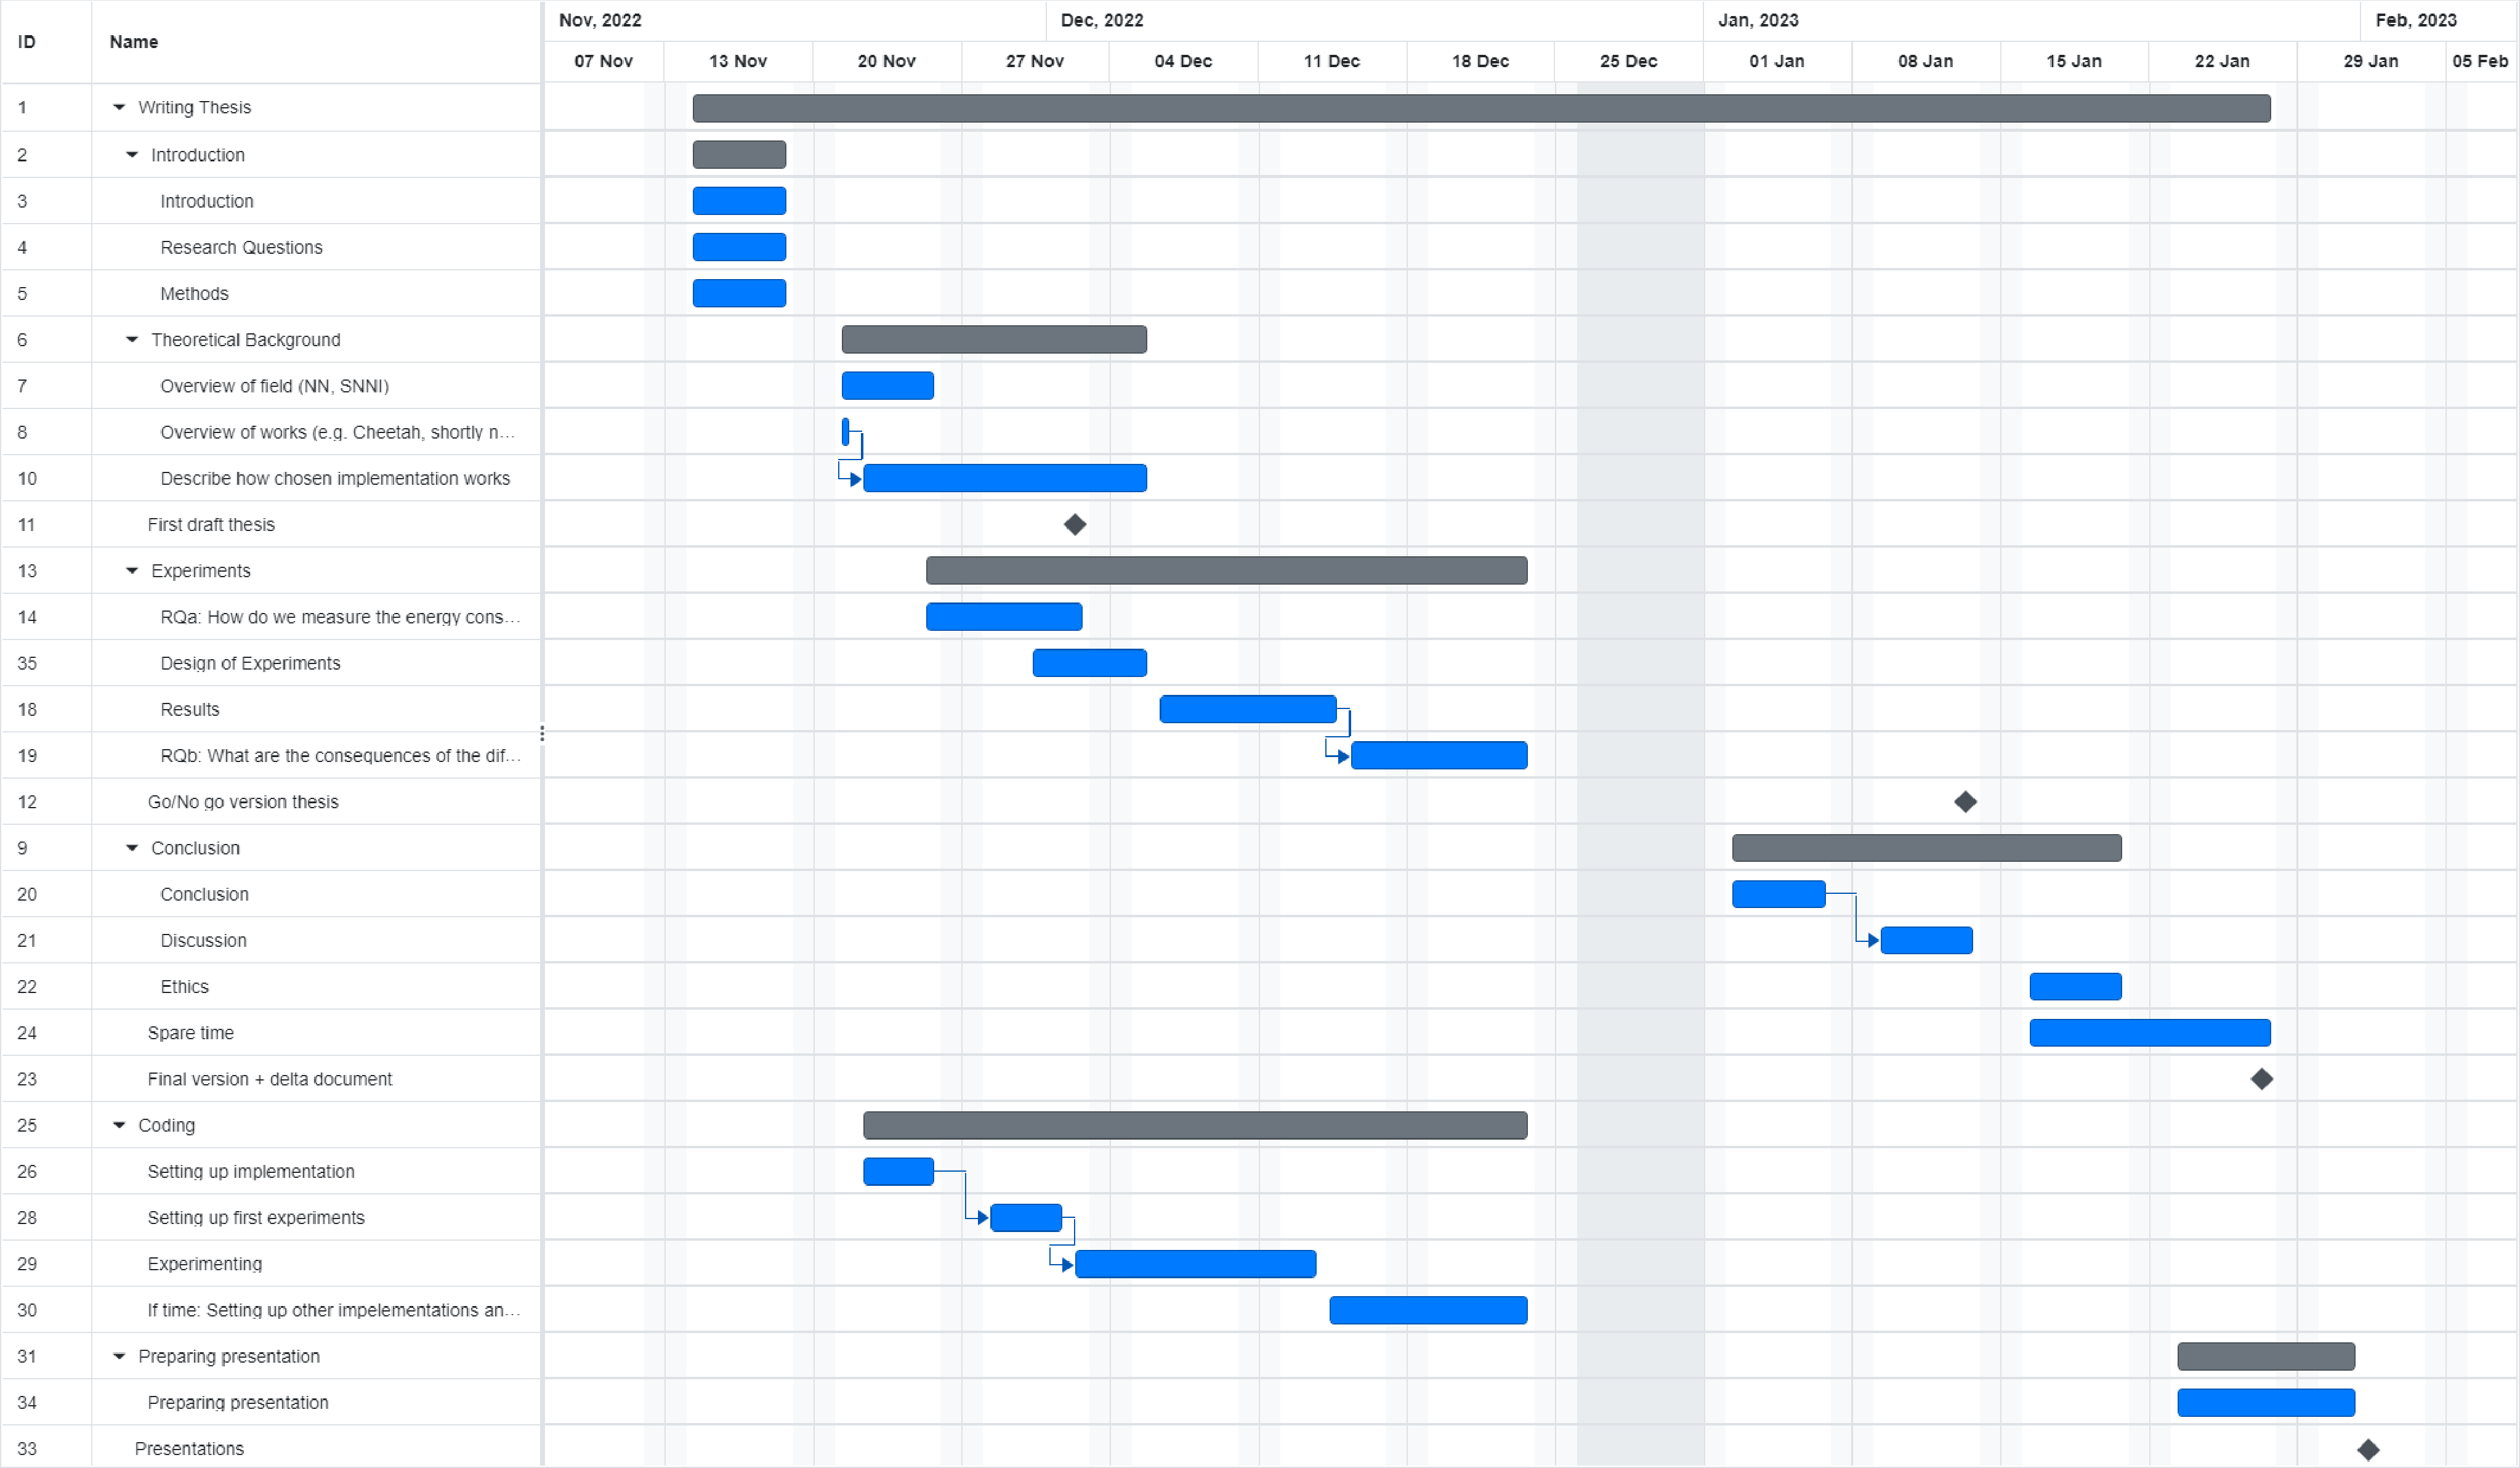
\includepdf[pages=-,angle=270]{Gantchart_Thesis.pdf}


% \subsectionauthor[Voornaam Achternaam]{Paragraaf met auteur}
% \lipsum[2-3]

%-------------------------------------------------------------------------------
%	REFERENTIES
%-------------------------------------------------------------------------------

\printbibliography

%-------------------------------------------------------------------------------
\end{document}